\documentclass[12pt, twoside]{article}
%\documentclass[12pt, twoside]{article}
\usepackage[letterpaper, margin=1in, headsep=0.2in]{geometry}
\setlength{\headheight}{0.6in}
%\usepackage[english]{babel}
\usepackage[utf8]{inputenc}
\usepackage{microtype}
\usepackage{amsmath}
\usepackage{amssymb}
%\usepackage{amsfonts}
\usepackage[nomessages]{fp} %\FPeval{\var-name}{2*sin(pi/6)}
\usepackage{siunitx} %units in math. eg 20\milli\meter
\usepackage{yhmath} % for arcs, overparenth command
\usepackage{tikz} %graphics
\usetikzlibrary{quotes, angles, arrows, arrows.meta}
\usepackage{pgfplots}
\usepgfplotslibrary{fillbetween}
\pgfplotsset{compat=1.16}
\usepackage{graphicx} %consider setting \graphicspath{{images/}}
\usepackage{parskip} %no paragraph indent
\usepackage{enumitem}
\usepackage{multicol}
\usepackage{venndiagram}

\usepackage{fancyhdr}
\pagestyle{fancy}
\fancyhf{}
\renewcommand{\headrulewidth}{0pt} % disable the underline of the header
\raggedbottom
\hfuzz=2mm %suppresses overfull box warnings

\usepackage{hyperref}

\fancyhead[LO]{La Scuola d'Italia / Dr.\ Huson / IB Math 12 \\* 11 November 2026}
\fancyhead[RO]{\fbox{\begin{minipage}{6cm}\footnotesize Nickname:\\[0.5cm]\end{minipage}}}
\fancyfoot[C]{\thepage}

\begin{document}
\subsubsection*{3.5 Pre-Quiz: Trigonometry Review}

A calculator is allowed. Give answers correct to three significant figures,
unless they are exact. Angles are in radians unless they are given in
degrees. Diagrams are not to scale.

\begin{enumerate}[itemsep=0.15cm]

%--- Problem 1: Double-angle identities: cos theta = 1/4 in quadrant IV, find sin theta, sin 2theta, cos 2theta exactly; show sin 2x/(1 + cos 2x) = tan x; hence tan theta [11 marks] ---
%--- Source: Original (AA SL 3.6, 3.5); complements 3-4PreT P3 (quadrant II, no double angle) ---
\item[1.] [Maximum mark: 11]

Let $\cos\theta = \dfrac{1}{4}$, where $\dfrac{3\pi}{2} < \theta < 2\pi$.

\begin{enumerate}[itemsep=0.1cm]
  \item Find the exact value of $\sin\theta$. \hfill [3]
  \item Find the exact value of $\sin 2\theta$. \hfill [2]
  \item Find the exact value of $\cos 2\theta$. \hfill [2]
  \item Show that $\dfrac{\sin 2x}{1 + \cos 2x} = \tan x$, for
  $\cos x \neq 0$. \hfill [3]
  \item Hence, or otherwise, find the exact value of $\tan\theta$. \hfill [1]
\end{enumerate}

\begin{tikzpicture}
  \draw (-0.6,0) rectangle (14.6,13.6);
  \foreach \y in {1,2,...,13} \draw[dotted] (0,\y)--(14.1,\y);
\end{tikzpicture}

\newpage

%--- Problem 2: Bearings: ship sails 12 km on 070 then 9 km on 170; show angle HAB = 80 deg; HB by cosine rule; bearing of B from H via sine rule; back bearing; area [12 marks] ---
%--- Source: Original (AA SL 3.2, 3.3); complements 3-4PreT P2 (SSS, ambiguous case) with bearings ---
\item[2.] [Maximum mark: 12]

\begin{minipage}[t]{0.56\linewidth}
A ship leaves harbour $H$ and sails $12\,\text{km}$ on a bearing of
$070^\circ$ to point $A$. It then sails $9\,\text{km}$ on a bearing of
$170^\circ$ to point $B$.
\end{minipage}
\hfill
\begin{minipage}[t]{0.4\linewidth}
\vspace{0pt}
\centering
\begin{tikzpicture}[scale=0.36]
  \coordinate (H) at (0,0);
  \coordinate (A) at (11.276,4.104);
  \coordinate (B) at (12.839,-4.759);
  \draw[->] (H) -- ++(0,4.5) node[above] {\footnotesize $N$};
  \draw[->] (A) -- ++(0,3.5) node[above] {\footnotesize $N$};
  \draw[thick] (H) -- (A) -- (B);
  \draw[dashed] (H) -- (B);
  \draw (0,1.6) arc (90:20:1.6);
  \node at (55:2.5) {\footnotesize $70^\circ$};
  \draw (11.276,5.404) arc (90:-80:1.3);
  \node at (13.9,4.4) {\footnotesize $170^\circ$};
  \fill (H) circle (3pt); \fill (A) circle (3pt); \fill (B) circle (3pt);
  \node[left] at (H) {$H$};
  \node[above left] at (A) {$A$};
  \node[below right] at (B) {$B$};
  \node[above left, inner sep=1pt] at (5.64,2.05) {\footnotesize $12\,\text{km}$};
  \node[left, inner sep=2pt] at (12.06,-0.33) {\footnotesize $9\,\text{km}$};
\end{tikzpicture}
\end{minipage}

\begin{enumerate}[itemsep=0.1cm]
  \item Show that $H\hat{A}B = 80^\circ$. \hfill [2]
  \item Find the distance $HB$. \hfill [3]
  \item Find the bearing of $B$ from $H$. \hfill [4]
  \item Write down the bearing of $H$ from $B$. \hfill [1]
  \item Find the area of triangle $HAB$. \hfill [2]
\end{enumerate}

\begin{tikzpicture}
  \draw (-0.6,0) rectangle (14.6,11.0);
  \foreach \y in {1,2,...,10} \draw[dotted] (0,\y)--(14.1,\y);
\end{tikzpicture}

\newpage

%--- Problem 3: Equations with double angles on [0, 2pi]: sin 2x = sin x (factorise, do not divide by sin x); cos 2x + 3cos x + 2 = 0 as a quadratic in cos x [11 marks] ---
%--- Source: Original (AA SL 3.8, 3.6); complements 3-4PreT P3(c) (linear equation in cos x) ---
\item[3.] [Maximum mark: 11]

Give your answers as exact multiples of $\pi$.

\begin{enumerate}[itemsep=0.1cm]
  \item Solve the equation $\sin 2x = \sin x$ for $0 \le x \le 2\pi$.
  \hfill [5]
  \item
  \begin{enumerate}[label=(\roman*), itemsep=0.05cm]
    \item Show that $\cos 2x + 3\cos x + 2 = 2\cos^{2}x + 3\cos x + 1$.
    \hfill [2]
    \item Hence solve the equation $\cos 2x + 3\cos x + 2 = 0$ for
    $0 \le x \le 2\pi$. \hfill [4]
  \end{enumerate}
\end{enumerate}

\begin{tikzpicture}
  \draw (-0.6,0) rectangle (14.6,16.6);
  \foreach \y in {1,2,...,16} \draw[dotted] (0,\y)--(14.1,\y);
\end{tikzpicture}

\newpage

%--- Problem 4: f(x) = 6 sin x cos x + 1 on [0, pi]: show f = 3 sin 2x + 1; period; range; sketch; solve f(x) = 2.5 exactly; values of k for exactly two solutions of f(x) = k [13 marks] ---
%--- Source: Original (AA SL 3.6, 3.7, 3.8); complements 3-4PreT P4 (cosine model) with a sine graph built from an identity ---
\item[4.] [Maximum mark: 13]

Let $f(x) = 6\sin x\cos x + 1$, for $0 \le x \le \pi$.

\begin{enumerate}[itemsep=0.1cm]
  \item Show that $f(x) = 3\sin 2x + 1$. \hfill [2]
  \item Write down the period of $f$. \hfill [1]
  \item Find the range of $f$. \hfill [2]
  \item Sketch the graph of $y = f(x)$ on the grid below. \hfill [3]
  \item Solve the equation $f(x) = 2.5$. Give your answers as exact
  multiples of $\pi$. \hfill [3]
  \item Find the values of $k$ for which the equation $f(x) = k$ has
  exactly two solutions. \hfill [2]
\end{enumerate}

\begin{center}
\begin{tikzpicture}[xscale=2.4, yscale=0.65]
  \foreach \x in {0.5,1,...,4} \draw[gray!40] (\x,-3) -- (\x,5);
  \foreach \y in {-3,...,5} \draw[gray!40] (0,\y) -- (4.2,\y);
  \draw[->] (0,0) -- (4.35,0) node[right] {$x$};
  \draw[->] (0,-3.2) -- (0,5.4) node[above] {$y$};
  \foreach \x/\l in {1/{\frac{\pi}{4}},2/{\frac{\pi}{2}},3/{\frac{3\pi}{4}},4/{\pi}}
    \node[below, fill=white, inner sep=1pt] at (\x,-0.12) {\small $\displaystyle\l$};
  \foreach \y in {-3,-2,-1,1,2,3,4,5}
    \node[left] at (0,\y) {\footnotesize $\y$};
\end{tikzpicture}
\end{center}

\begin{tikzpicture}
  \draw (-0.6,0) rectangle (14.6,8.4);
  \foreach \y in {1,2,...,8} \draw[dotted] (0,\y)--(14.1,\y);
\end{tikzpicture}

\end{enumerate}
\end{document}
